\documentclass[tikz,border=7pt]{standalone}
\usepackage{pgfplots}
\pgfplotsset{compat=1.18}
\begin{document}
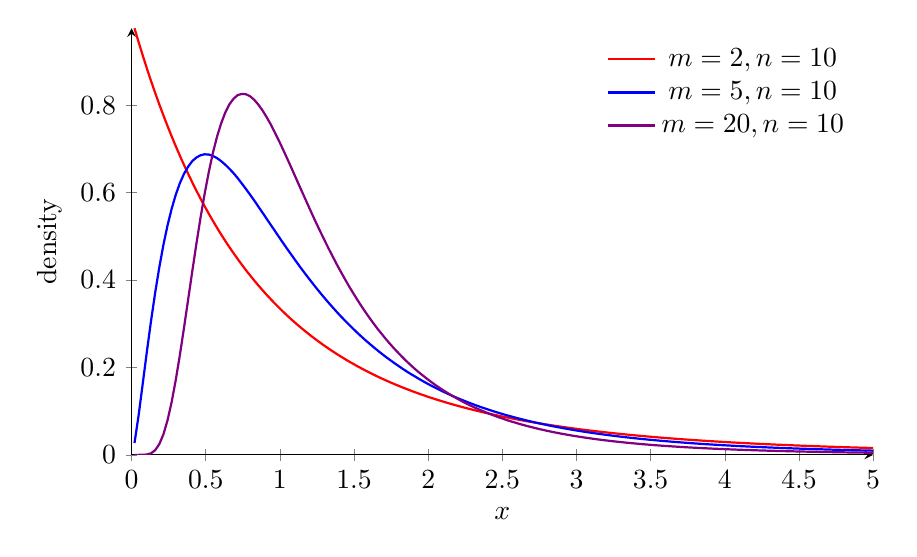
\begin{tikzpicture}
\begin{axis}[width=11cm,height=7cm,axis lines=left,xmin=0,xmax=5,ymin=0,samples=180,xlabel={$x$},ylabel={density},legend style={draw=none}]
\addplot[red,thick,domain=.02:5] {x^0*(1+.2*x)^(-6)}; \addlegendentry{$m=2,n=10$}
\addplot[blue,thick,domain=.02:5] {10.3683675*x^1.5*(1+.5*x)^(-7.5)}; \addlegendentry{$m=5,n=10$}
\addplot[violet,thick,domain=.02:5] {10250240*x^9*(1+2*x)^(-15)}; \addlegendentry{$m=20,n=10$}
\end{axis}
\end{tikzpicture}
\end{document}
